\section{Übersicht}
\subsection{Einsatzgebiet}
Öffentlicher Personennahverkehr bezeichnet den \glqq{} räumlichen Bereich zur Beförderung von Personen im Berufs-,
Ausbildungs-, Einkaufs- und sonstigen alltäglichen Verkehr mit Fahrzeugen des Straßen-, Schienen- und Schiffsverkehrs (Fähren) im Linienverkehr.
\grqq{} \cite{Dr.FriedrichvonStackelbergDr.RobertMalina.2018}
Die Einsatzgebiete von Fahrgastüberwachung betreffen alle dem entsprechenden Verkehrsbetrieb zugehörigen Gebiete, in welchen sich Personen aufhalten.
Dies umfasst also die Haltestellen sowie die Verkehrsmittel selbst.
\subsection{Rechtliche Rahmenbedingungen}
Die rechtliche Grundlage für die Fahrgastüberwachung ist durch §4 Bundesdatenschutzgesetz Abs. 1 S. 2 \glqq{} Videoüberwachung öffentlich zugänglicher Räume\grqq{}
gegeben. Genauer heißt es dort:\\
\glqq{}Bei der Videoüberwachung von
\begin{enumerate}
    \item öffentlich zugänglichen großflächigen Anlagen, wie insbesondere Sport-,\\ Versammlungs- und Vergnügungsstätten, Einkaufszentren oder Parkplätzen, oder
    \item Fahrzeugen und öffentlich zugänglichen großflächigen Einrichtungen des öffentlichen Schienen-, Schiffs- und Busverkehrs
\end{enumerate}
gilt der Schutz von Leben, Gesundheit oder Freiheit von dort aufhältigen Personen als ein besonders wichtiges Interesse.\grqq{} \cite{Bundestag.2018}\\
Ebenfalls die Fahrgastüberwachung betreffend ist die europäische Datenschutzgrundverordnung bezüglich Artikel 6 \glqq{}Rechtmäßigkeit der Verarbeitung\grqq{},
Artikel 13, 14\glqq{}Informationspflicht\grqq{} und Artikel 17 \glqq{}Recht auf Löschung\grqq{} \cite{EuropaischeUnion.}

\subsection{Architektur}
In Abbildung~\ref{fig:architektur} wird der Systemaufbau dargestellt. Hierbei wird unterschieden zwischen dem lokalen Aufbau, der an den Fahrzeugen und Haltestellen
anzufinden ist. Über ein Netzwerk ist jedes lokale System mit der zentralen Leitstelle verbunden.

Ein lokales System hat in der Regel mehrere Kameras (analog oder digital) verbaut. Das Bild analoger Kameras muss vor Anbindung an das Netzwerk digitalisiert werden.
Optional in den lokalen System sind eine Anzeige für z.B. deb Fahrer des Busses, sowie Mikrofone, welche in den Kameras integriert sein können.

In der zentralen Verwaltung stehen die Server, welche die Videoaufnahmen verwalten sowie das \glqq{}Langzeit-Archiv\grqq{}. In diesem werden die Aufnahmen bis zur Löschung aufbewahrt.
Über den Dauer bis zur Löschung der Daten heißt bisher Uneinigkeit, gemäß § 27 Bundespolizeigesetz (BPolG) ist eine Speicherung von bis zu 30 Tagen zulässig. In  §6b Abs. 5 BDSG
steht dem die unweigerliche Löschung der Daten gegenüber. In der \glqq{}Orientierungshilfe zur Videoüberwachung\grqq{} der Datenschutzbeauftragten von Niedersachsen wird eine maximale
Speicherdauer von 48 Stunden angegeben\cite{DanielaWindelband.20.April2016}. Neben der Darstellung der Videos sind auch technische Möglichkeiten zur Auswertung der Videos geschaffen.
Auswertung umfasst nicht automatisch die automatische Analyse der Daten, sondern beschreibt vielmehr das Betrachten und Beurteilen dieser durch einen Mitarbeiter.

\begin{figure}[ht]
    \begin{center}
        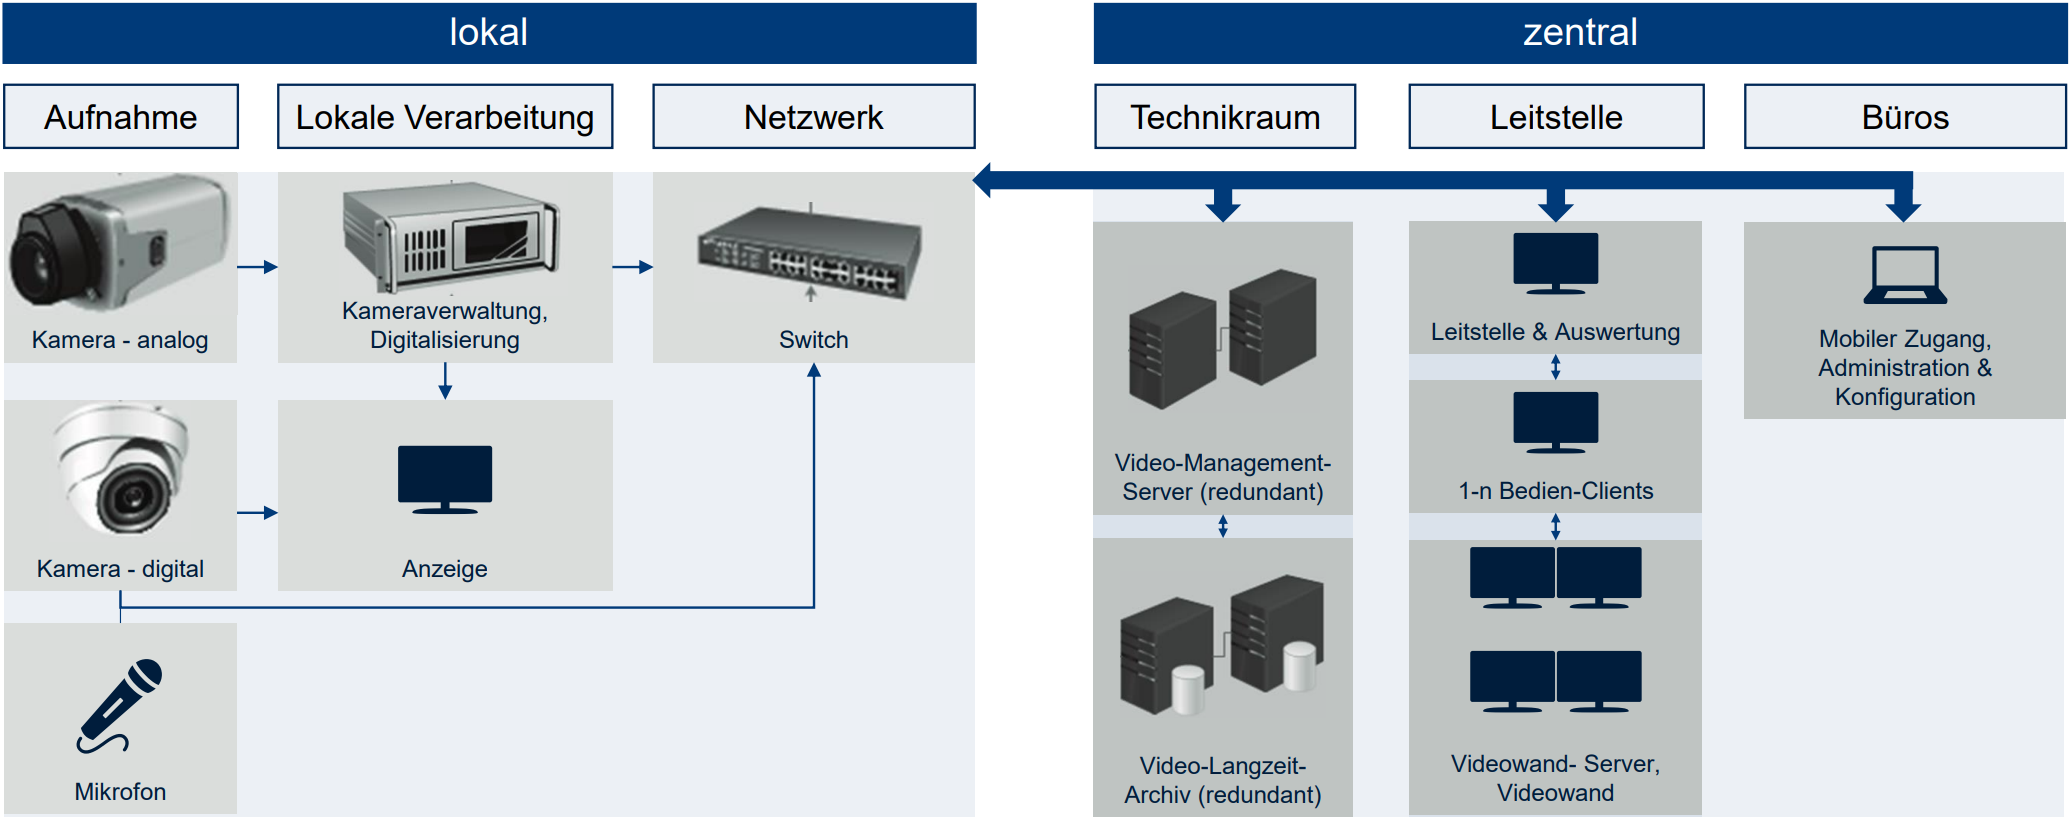
\includegraphics[width= 1\textwidth]{Bilder/architektur.png}
        \caption{Aufbau eines typischen Systems \cite{LandesbeauftragtefurdenDatenschutzBadenWurttemberg.2015}}
        \label{fig:architektur}
    \end{center}
\end{figure}
Die genaue Implementierung eines Systems kann abweichen, wichtig sind aber die Aspekte der Netzwerkübertragung und zentralen Auswertungsstelle für mehrere Kamerabilder.
